% !TeX spellcheck = en_GB
\section{Numerics}
\subsection{High Performance Computations}
It is important to make the program as fast as possible.
Indeed, the faster the program goes, the more data it will generate (within the same amount of time).
This data will be used for numerical analysis and we will also use it for interpretation.
Therefore, with more data, we have more knowledge, and we can make smarter guesses.

There are two main ways to make a program faster:
use a better algorithm, or 
use a faster implementation.
A better algorithm means, for example, test factors only up to square root (in the case of primality a test).
A better implementation simply means optimisation inside the computer (i.e. on operations that are made, types that are used...).
We will try to optimise both.

\subsubsection{Algorithm Optimisation}
\label{algorithmOptimisation}
We can optimize an algorithm by optimizing (decreasing) the number of operations, or by using mathematical scheme (usually cancellations).
\paragraph{Optimize instructions}
Optimizing instructions usually comes through optimizing loops (stopping loops as soon as possible, avoiding extra loops...).
For example, the following two algorithms create the same list of coefficients for the $q$-series of $\Delta$.

\textbf{\textit{Algorithm 1:}}
\begin{algorithmic}
	\color{CodeColor}
	\Require $L \geq 1$
	\State{$f \leftarrow zeros(L)$}\Comment{Empty list of length $L$}
	\State{n=0}
	\While{$n < L$}
		\If{$(\sqrt{n}-1) \% 2 = 0$}
			\State{$f[n]=1$}
		\EndIf
	\EndWhile
\end{algorithmic}

\textit{\textbf{Algorithm 2:}}
\begin{algorithmic}
	\color{CodeColor}
	\Require $L \geq 1$
	\State{$f \leftarrow zeros(L)$}\Comment{Empty list of length $L$}
	\State{$id=1$}
	\State{$i=1$}
	\While{$id < L$}
		\State{$f[id] = 1$}
		\State{$i += 2$}
		\State{$id = i^2$}
	\EndWhile
\end{algorithmic}

However, the second algorithm is significantly more efficient: the loop is faster as it only goes through odd squares instead of all numbers, and it has no condition to check.
The algorithms may be \textit{harder} to understand, but it in fact is \textit{better} (in terms of performance).

\paragraph{Mathematical ruse}
As we are working modulo 2, there are obviously many cancellations, which will make the calculations \textit{faster}.
It is an opportunity we shouldn't miss to make the algorithms \textit{stronger}.
% harder, better, faster, stronger
\subsubsection{Implementation Approach}
As explained above, investigations on which tool will be the more suitable for the computations is an important part.
Of course, the best would be to find a programming language that can already deal with modular forms modulo two.
Unfortunately, this (yet) doesn't exist.
There are packages that have modular forms implemented, but none with modular forms modulo two specifically.
The goal of looking at modulo two is to conclude more than what we know in general.
So using what has already been done in general to make computations modulo two won't give any thing interesting.

We realize that there is no other way than just creating a package for modular forms modulo two on our own.
In fact, this is what we will do later, but before, we want to determine the tools to build this package.
Modular forms modulo 2 come from maths, so it makes sense to use a \href{https://en.wikipedia.org/wiki/High-level_programming_language}{high level programming language}.
For scientific computing nowadays, there are two main \href{https://en.wikipedia.org/wiki/Open-source_model}{open source} languages: \href{https://en.wikipedia.org/wiki/Python_(programming_language)}{Python} and \href{https://en.wikipedia.org/wiki/Julia_(programming_language)}{Julia}.
Each having various packages to work with.

We will test a selection of major ones.

\subsubsection{Choice of Implementation}
Now it is time to wonder how to represent modular forms modulo 2.
We have seen above that a modular form modulo 2 in fact have two representations: one as an infinite $q$-series, and one as a finite $\Delta$-polynomial.
As we want (later on) to compute Hecke operators of these forms, we will need, at some point to use the $q$-series representation.
In fact, this will be one of the crucial points, since it is an infinite series.
The way we represent infinite objects in computers, which have only a finite amount of components (memory addresses, say), is to only store informations up to a cutting point.
This is equivalent (somewhat) to the asymptotic notation in mathematics.
In the case of $q$-series of modular forms, we will store only the few first hundred/thousand/million coefficients.

This means that we will represent a modular form via its $q$-series, witch will be stored as a list.
We investigate the best ways (timewise) to do basic operations to decide what technology to use.
The operations tested are creating the $q$-series of $\Delta$, and squaring it (both storing coefficients up to some power \texttt{LENGTH}, the length of the list used).

There are various techniques to store lists in a computed, the main ones are continuous list, linked list, and sparse list.
Continuous and linked lists can be aggregated as dense lists.

\paragraph{Dense Technique}
Dense storage means that we store each values of the list (next to each other, or with a link to the next).
No element of the list is skipped.
There are various ways to implement this technique:
\subparagraph{Pure Python}
Using the Python language, this is the most elementary way to go.
It represents all the $q$-coefficients with the default linked list python object.
\begin{minted}{python}
def delta(LENGTH):
	f = [0 for i in range(LENGTH)]
	indice = 1
	i = 1
	while indice<LENGTH:
		f[indice] = 1
		i += 2
		indice = i**2
	return f

def square(f):
	f_sq = [0 for i in range(len(f))]
	i = 0
	while 2*i < len(f):
		if f[i]:
			f_sq[2*i] = 1
		i += 1
	return f_sq
\end{minted}
\subparagraph{NumPy Python}
\href{https://fr.wikipedia.org/wiki/NumPy}{NumPy} is the most well known scientific computing library for Python.
It interfaces with C objects to provide very fast features (such as lists).
\begin{minted}{python}
import numpy as np

def delta(LENGTH):
	f = np.zeros(LENGTH, dtype=np.int8)
	indice = 1
	i = 1
	while indice<LENGTH:
		f[indice] = 1
		i += 2
		indice = i**2
	return f

def square(f):
	f_sq = np.zeros(len(f), dtype=np.int8)
	i = 0
	while 2*i < len(f):
		if f[i]:
			f_sq[2*i] = 1
		i += 1
	return f_sq
\end{minted}
\subparagraph{Dense Julia}
Julia is well-known as both high level and very fast language.
Julia naturally supports lists, that we can use to represent modular forms.
\begin{minted}{julia}
function delta(LENGTH)
	f = zeros(Int8, LENGTH)
	indice = 2
	i = 1
	while indice < LENGTH
		f[indice] = 1
		i += 2
		indice = i^2 + 1
	end
	return f
end

function square(f)
	f_sq = zeros(Int8, length(f))
	i = 1
	while 2 * i - 1 < length(f)
		if f[i] == 1
			f_sq[2 * i - 1] = 1
		end
		i += 1
	end
	return f_sq
end
\end{minted}

\paragraph{Sparse Technique}
As all coefficients of the $q$-series are just $0$ or $1$, and that most of the time, they are $0$, we can represent a modular forms by storing only the coefficients for which it is non-zero.
This method is (storing only non-zero values) is known as \href{https://en.wikipedia.org/wiki/Sparse_matrix}{sparse representation}.
We can implement this technique in both Python and Julia:
\subparagraph{Sparse Python}
We can adapt the previous code to use Python's linked lists as index of a sparse list.
Note that in general, we would need a second list to store values, but there ar only $0$s and $1$s, we can take as convention that all stored indices have value $1$ and all non-store have value $0$. 
\begin{minted}{python}
def delta(LENGTH):
	f = []
	indice = 1
	i = 1
	while indice < LENGTH:
		f.append(indice)
		i += 2
		indice = i**2
	return (f, LENGTH)

def square(form):
	f_sq = []
	f = form[0]
	for n in f:
		if 2*n-1 <= form[1]:
			f_sq.append(2*n-1)
	return (f_sq, form[1])
\end{minted}
\subparagraph{Sparse Julia}
Julia has a very convenient built-in sparse module.
This is particularly interesting, since the built-in type already have nice methods.
\begin{minted}{julia}
using SparseArrays: SparseVector, spzeros

function delta(LENGTH)
	f = spzeros(Int8, LENGTH)
	indice = 2
	i = 1
	while indice <= f.n
		f[indice] = Int8(1)
		i += 2
		indice = i^2 + 1
	end
	return f
end

function square(f)
	f_sq = spzeros(Int8, f.n)
	for n in f.nzind
		if 2n - 1 <= f_sq.n
			f_sq[2n - 1] = 1
		end
	end
	return f_sq
end
\end{minted}
\paragraph{Speed Comparison}
We can now compare the speed of each implementation to compute $q$-series.
If we do that for various number of coefficients, we may obtain a graph of the following type (it is sightly dependent on the machine that execute the code, but the shape remains).

\includegraphics{speed_comparison_delta}

For small computations, the implementation doesn't make a big difference.
However, for large computations, it seems that the sparse methods do better.
It makes sense, since sparse representations are typically used for objects with more than 95\% of zeros, which is the case for modular forms modulo 2.

For a more precise analysis, we now compare the speed of each implementation to compute $q$-series of $\Delta$ and $\Delta^2$
\footnote{$\Delta^2$ itself isn't part of our space $\mathcal{F}$, but it will be useful as we will compute $\Delta^{2k+1} = \Delta^{2k-1}\cdot \Delta^2$. So it makes sense to be concerned about it.}.
The following table is obtained for $10^6$ coefficients computed (i.e. up to $q^{10^6}$).
Note that $\mathcal{O}(q^{10^6})$ will be standard for the rest of this paper.

\begin{center}
	\begin{tabular}{r||l|l}
		 & $\Delta$ & $\Delta^2$\\
		\hline\hline
		Pure Python   & 0.08263147 & 0.26249526 \\
		NumPy Python  & 0.00138761 & 0.16163688 \\
		Dense Julia   & 0.000648   & 0.001698   \\
		Sparse Python & 0.00095099 & 0.00134479 \\
		Sparse Julia  & 0.000021   & 0.000034   \\
	\end{tabular}
\end{center}

From this table, it is clear that the fastest implementation is the one using sparse lists (so called "sparse vectors") in Julia.
Therefore, we will use this technique.
It is nice to remark that the Pure Python implementation was 7720 times slower than the Sparse Julia one.
We see here the importance of choosing the right tool to implement an algorithm.

This ratio would even be greater considering the bad algorithm presented before \ref{algorithmOptimisation}.



\subsection{Creating the library}
It is clear now that the code should be done with Julia and it's Sparse objects.
Now, as all the library should be created from the beginning, it is a good idea to pack all of it in a Julia module.
Doing so, no code will be repeated for each small task.
\paragraph{Code Architecture}
The code will be divided in a many files, for convenience.

\begin{forest}
	for tree={
		font=\ttfamily,
		grow'=0,
		child anchor=west,
		parent anchor=south,
		anchor=west,
		calign=first,
		edge path={
			\noexpand\path [draw, \forestoption{edge}]
			(!u.south west) +(7.5pt,0) |- node[fill,inner sep=1.25pt] {} (.child anchor)\forestoption{edge label};
		},
		before typesetting nodes={
			if n=1
			{insert before={[,phantom]}}
			{}
		},
		fit=band,
		before computing xy={l=15pt},
	}
	[text1
	[text1.1
	[text1.1.1]
	[text1.1.2]
	[text1.1.3]
	]
	[text1.2
	[text1.2.1]
	[text1.2.2]
	]
	]
\end{forest}

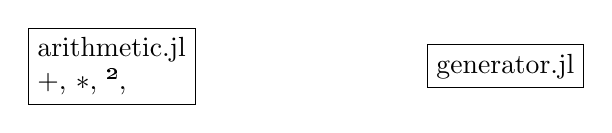
\begin{tikzpicture}

\node[draw,align=left] at (0,0) {arithmetic.jl\\$+$, $*$, ², $^{\boxed{}}$};
\node[draw] at (5,0) {generator.jl};


\end{tikzpicture}



\tikzset{
	state/.style={
		rectangle,
		rounded corners,
		draw=black, very thick,
		minimum height=4.2cm,
		minimum width=3.8cm,
		inner sep=2pt,
		text width=3.7cm,
	},
}

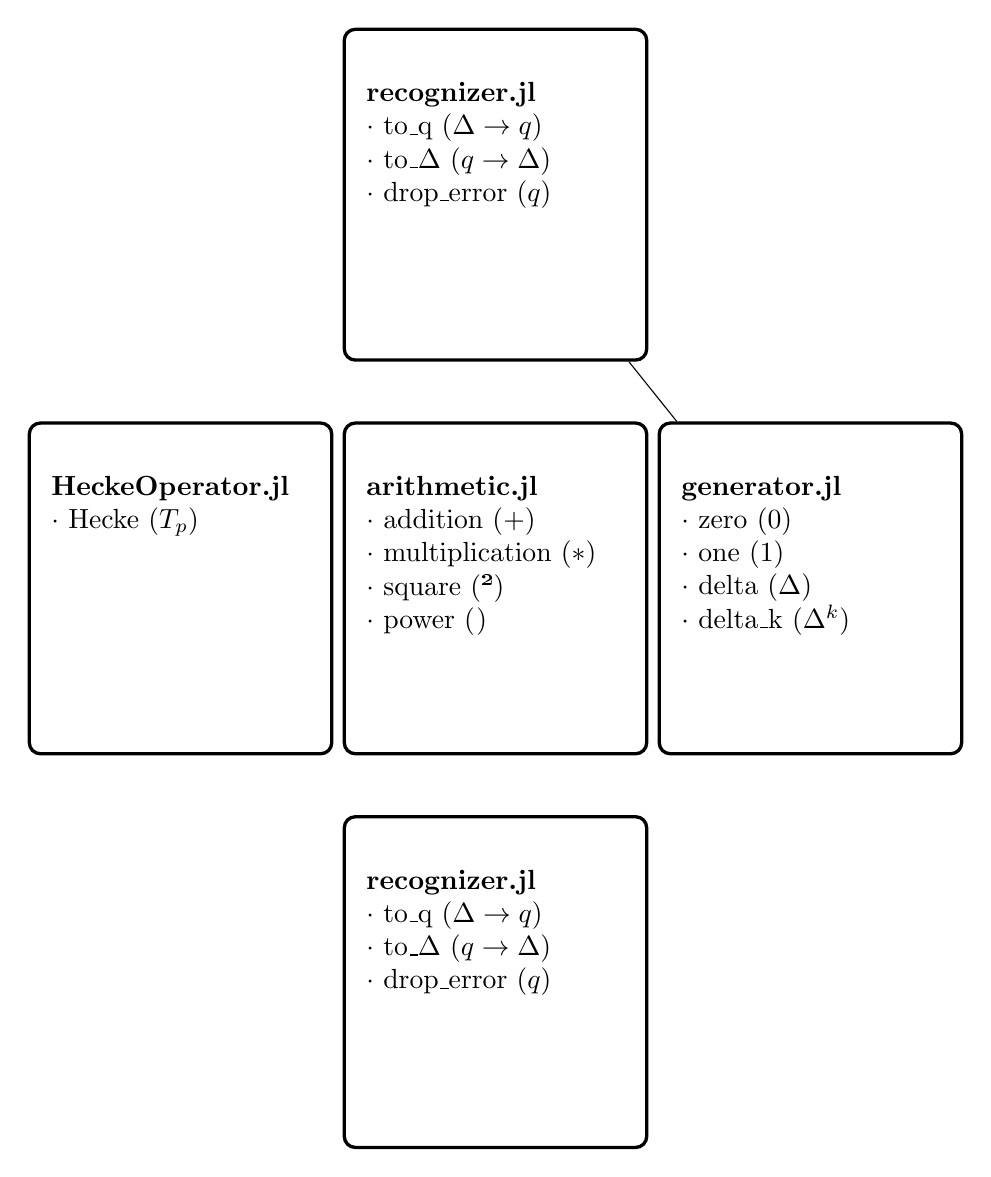
\begin{tikzpicture}
\coordinate(center) at (0,0);
\node[state] (arithm) at (center){
	\begin{tabular}{l}
		\textbf{arithmetic.jl}\\
		$\cdot$ addition ($+$)\\
		$\cdot$ multiplication ($*$)\\
		$\cdot$ square (²)\\
		$\cdot$ power (${}^{\boxed{}}$)\\
		\\\\
	\end{tabular}
};
\node[state, right of = center, node distance=4cm] (gene){
	\begin{tabular}{l}
	\textbf{generator.jl}\\
	$\cdot$ zero ($0$)\\
	$\cdot$ one ($1$)\\
	$\cdot$ delta ($\Delta$)\\
	$\cdot$ delta\_k ($\Delta^k$)\\
	\\\\
	\end{tabular}
};
\node[state, left of = center ,node distance=4cm] (Hecke){
	\begin{tabular}{l}
	\textbf{HeckeOperator.jl}\\
	$\cdot$ Hecke ($T_p$)\\
	\\
	\\
	\\
	\\\\
	\end{tabular}
};
\node[state, below of = center ,node distance=5cm] (reco){
	\begin{tabular}{l}
	\textbf{recognizer.jl}\\
	$\cdot$ to\_q ($\Delta \to q$)\\
	$\cdot$ to\_$\Delta$ ($q \to \Delta$)\\
	$\cdot$ drop\_error ($q \circlearrowleft$)\\
	\\
	\\\\
	\end{tabular}
};
\node[state, above of = center ,node distance=5cm] (reco){
	\begin{tabular}{l}
	\textbf{recognizer.jl}\\
	$\cdot$ to\_q ($\Delta \to q$)\\
	$\cdot$ to\_$\Delta$ ($q \to \Delta$)\\
	$\cdot$ drop\_error ($q \circlearrowleft$)\\
	\\
	\\\\
	\end{tabular}
};
\path (gene) edge (reco);


\end{tikzpicture}




\paragraph{Published}

\paragraph{Online Library}





\subsection{Finding coefficients of Hecke operators}

We want to find the coefficients $a_{ij}$ such that $$\sum_{i, j} a_{ij} T_3^iT_5^j = T_p$$
(with $a_{ij} \in \mathbb{F}_2$).

Let $k\geq 1$ an integer.
Then there exists an integer $N(k)>0$ such that,
for all pairs of non-negative integers $(i, j)$ with $i+j \geq N(k)$,
we have $T_3^{i}T_5^{j}|\Delta^k = 0$.

This allows us to write:
$$\sum_{i+j < N(k)} a_{ij} T_3^iT_5^j|\Delta^k= T_p|\Delta^k \qquad (*)$$

Now, suppose that we want to calculate the table of the $a_{ij}(p)$ for $p \in \primes$:
\begin{enumerate}
    \item Take an odd power for $\Delta$ (say $k$, we usually start with the smallest: 1 and the increase gradually)
    \item Plug $\Delta^k$ in the equation above, ie:
    \item Calculate $T_3^iT_5^j|\Delta^k \forall i+j < N(k)$
    \item Calculate $T_p|\Delta^k \forall i+j < N(k)$
    \item Equate both sides of $(*)$, if not zero (which unfortunately happens often), use the equation to deduce $a_{ij}(p)$
\end{enumerate}

[How much of the algorithm is there? too much? too little? I could develop much more on how everything is calculated: how I go back and forward between $q$ and $\Delta$ representations of modular forms to both be efficient in calculations and catch up the error in numerical approximation, what techniques are used for speed, argue the implementation choices, describe how the code is split, etc... I could write at least  pages on all of that, but is it the point of a math paper?]
